%==============================================================================
%== template for LATEX poster =================================================
%==============================================================================
%
%--A0 beamer slide-------------------------------------------------------------
\documentclass[final]{beamer}
\usepackage[orientation=portrait,size=a0,
            scale=1.25         % font scale factor
           ]{beamerposter}
           
\geometry{
  hmargin=2.5cm, % little modification of margins
}

%
\usepackage[utf8]{inputenc}

\linespread{1.25}

%
%==The poster style============================================================
\usetheme{sharelatex}

%==Title, date and authors of the poster=======================================
\title
[Des enveloppes convexes, 2017-2018, Dijon, France] % Conference
{ % Poster title
Enveloppe convexe de points dans le plan Euclidien usuel
}

\author{ % Authors
Andrew LENC, Axel LE BOT
}
\institute
[Université de Bourgogne] % General University
{
ESIREM, France\\[0.3ex]
}
\date{\today}



\begin{document}
\begin{frame}[t]
%==============================================================================
\begin{multicols}{3}
%==============================================================================
%==The poster content==========================================================
%==============================================================================

\section{Introduction}

Dans un espace vectoriel E normé réel de dimension finie, on peut dire d'une partie C de E qu'elle est convexe si pour toutes paires de points pris dans C, le segment qui les connecte est entièrement contenu dans C.

L'enveloppe convexe d'un ensemble de points fini est aussi l'ensemble de toutes les combinaisons convexes de ces points. C'est-à-dire qu'on peut réaliser une moyenne pondérée de ces points (tant que la somme des coefficients est égale à 1) et obtenir un point contenue dans l'enveloppe convexe, par conséquent l'enveloppe convexe sera l'ensemble de toutes ces moyennes. Ceci est décrit par la formule (1).
\begin{equation}
Conv(S) = \left \{  \sum_{i=1}^{|S|} \alpha_{i}x_{i} \left | (\forall i : \alpha_{i} \geqslant 0) \wedge  \sum_{i=1}^{|S|} \alpha_{i} = 1 \right \}
\end{equation}

Il est demandé dans le sujet de déterminer l'enveloppe convexe d'un nombre variable de points, dans le langage C ou C++, à l'aide de la bibliothèque OpenGL pour l'affichage.

\section{Algorithmes}

De nombreux algorithmes ont été écrits afin de résoudre le problème des enveloppes convexes, nous allons examiner le fonctionnement des plus connus, puis identifier et clarifier celui qui a été retenu afin de réaliser ce projet. On traitera, bien entendu, uniquement des algorithmes utilisés dans le cas planaire précisé par l'énoncé.
\subsection{Jarvis}
La marche de Jarvis consiste à envelopper les points en trouvant un point appartenant à l'enveloppe, puis à continuer le long de celle-ci en cherchant le segment suivant ayant l'angle minimal avec le précédent. Il s'agit d'une des méthodes les plus intuitives, puisque comparable à envelopper les points dans, par exemple, du papier cadeau.

\subsection{Graham}
Le parcours de Graham trouve d'abord le point de plus petite ordonnée (départagé par l'abscisse la plus basse), puis il trie les points en fonction de l'angle du segment qui les relie à P et l'axe des abscisses. Ensuite, pour chaque triplet de points successifs dans le tableau précédemment créé, l'algorithme détermine s'il s'agit d'un "tournant à gauche" ou "à droite", et exclut le point du milieu dans le cas d'un tournant à gauche (puisque les points sont parcouru dans le sens horaire).

\subsection{QuickHull}
L'algorithme détermine d'abord les points avec les abscisses la plus basse et la plus haute, puisque ceux-ci font toujours partie de l'enveloppe convexe, puis il divise l'ensemble des points en deux ensemble de chaque côté de l'axe, ceux-ci seront traités de façon récursive. Pour chaque partie, l'algorithme détermine le point le plus éloigné de l'axe, grâce à celui-ci, on peut déterminer un triangle avec les deux autres points déterminés plus tôt et conclure que les points à l'intérieur du triangle ne font pas partie de l'enveloppe. On répète ensuite cette étape sur les deux nouveaux axes obtenus par les ligne du triangle. L'algorithme finit lorsque le tableau de points à traiter est vide.

\subsection{Chan}

Il s'agit d'un des algorithmes les plus complexes dans l'exécution, mais un des plus optimisés. Il consiste à diviser l'ensemble de points en plus petits ensemble et à en calculer l'enveloppe convexe grâce au parcours de Graham, puis à calculer l'enveloppe convexe des enveloppes calculées grâce à la marche de Jarvis.

\subsection{Andrew}
Cet algorithme trie d'abord les points par leur abscisees, et les départage par leur ordonnée, puis construit deux "coques", une supérieure, qui démarre au point le plus à gauche et finit au point le plus à droite, et une inférieure qui constitue le reste de l'enveloppe. Dans chaque coque, l'algorithme détermine les points à choisir en parcourant la liste triée, et en comparant les angles des segments, de manière similaire à la marche de Jarvis.

\vskip1ex
\begin{figure}
\centering
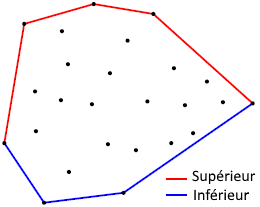
\includegraphics[width=0.99\columnwidth]{UpperAndLowerConvexHulls.png}
\caption{Principe des deux "coques" de l'algorithme de Andrew }
\end{figure}
\vskip2ex

\subsection{Comparatif}
On compare la complexité des algorithmes les plus connus. n étant le nombre de points que doit traité l'algorithme, alors que h est le nombre de points finalement contenus dans l'enveloppe convexe. La première ligne décrit la complexité théorique, tandis que la seconde précise la pire complexité à laquelle on peut s'attendre, en fonction de la nature des points à traiter (symétrie, groupement, etc).
\vskip1ex
\begin{table}
\centering
\caption{Comparatif des complexité des différents algorithmes}
\begin{tabular}{ccccc}
\hline\hline
Jarvis & Graham & Chan & QuickHull & Andrew\\
\hline
o(hn) & O(n log n) & O(n log h) & O(n log n) & O(n log n)\\
o(n²) & O(n log n) & O(n log n) & O(n log n) & O(n log n)\\
\hline\hline
\end{tabular}
\end{table}
\vskip2ex

\vfill\null
\columnbreak
\section{Autour du programme}
(Le programme n'étant pas encore fini, le reste du texte sert de remplissage pour garder une mise en page correct) Lorem ipsum dolor sit amet, consectetur adipiscing elit. Proin dictum libero at efficitur facilisis. Ut vitae malesuada nibh. Cras sed pharetra diam. In hac habitasse platea dictumst. Duis venenatis, eros vitae aliquam hendrerit, nunc augue ultrices ex, vitae mollis nisl sem in felis. Donec euismod lectus nec nisi tempus tempor. Nam eget gravida ipsum. Praesent tristique eget elit quis mattis. Sed in enim ullamcorper, rutrum ligula ac, vestibulum ex.

Vestibulum ante ipsum primis in faucibus orci luctus et ultrices posuere cubilia Curae; In a maximus sapien. Donec leo dolor, pulvinar vel convallis eget, vulputate quis neque. Praesent hendrerit, risus a vehicula tincidunt, dui lectus bibendum elit, a dictum risus ligula vel mi. Pellentesque quis ullamcorper lectus. Aliquam eget nisl a tortor ornare placerat. Ut rutrum vehicula tristique. Cras aliquam et turpis a ultrices. Aliquam luctus, tellus id sodales laoreet, urna diam posuere erat, quis condimentum risus odio at massa. Mauris interdum ultricies bibendum.

Vestibulum ante ipsum primis in faucibus orci luctus et ultrices posuere cubilia Curae; Fusce magna ante, eleifend quis aliquam non, ornare eget massa. Mauris tristique, lacus eget volutpat suscipit, nunc elit viverra odio, nec viverra velit neque eu augue. Vivamus arcu risus, euismod non pulvinar ut, bibendum ac metus. Donec fringilla leo sit amet suscipit elementum. Morbi sit amet faucibus risus, pharetra hendrerit justo. Morbi tristique egestas massa non suscipit. Mauris risus ipsum, mattis id sagittis in, accumsan at justo. In finibus dapibus orci quis viverra. Aenean euismod mauris et mi auctor congue. Pellentesque lacinia quis ipsum ut lacinia. Aenean in iaculis purus, malesuada auctor elit. Aenean quis efficitur sapien.

Duis et metus sem. Duis varius, purus et pretium scelerisque, est ipsum tempus nibh, a rutrum velit tellus vitae nibh. Donec ornare tellus non pulvinar laoreet. Donec faucibus odio lectus, nec pretium arcu efficitur quis. Morbi orci magna, imperdiet eget tincidunt vitae, viverra eget magna. Nullam placerat, nibh vitae lobortis cursus, magna sem posuere arcu, sit amet laoreet elit mi in urna. Pellentesque pretium urna eget nisl pharetra dapibus.



%==============================================================================
%==End of content==============================================================
%==============================================================================

%--References------------------------------------------------------------------

\subsection{Bibliographie}

\begin{thebibliography}{99}
\bibitem{ref1} Université d'Angers, \textit{http://enseignement.math.univ-angers.fr/documents/MEF1_geom1/convexite.pdf}

\bibitem{ref2} Page sur le parcours de Graham de Wikipedia, \textit{https://fr.wikipedia.org/wiki/Parcours_de_Graham}

\bibitem{ref3} Page sur la marche de Jarvis de Wikipedia, \textit{https://fr.wikipedia.org/wiki/Marche_de_Jarvis}

\bibitem{ref4} Page sur l'algorithme QuickHull de Wikipedia en anglais, \textit{https://en.wikipedia.org/wiki/Quickhulln}

\bibitem{ref5} Page sur l'algorithme de Chan de Wikipedia, \textit{https://fr.wikipedia.org/wiki/Algorithme_de_Chan}

\bibitem{ref6} Page sur l'algorithme Monotone Chain de Wikibook, \textit{https://fr.wikipedia.org/wiki/Algorithme_de_Chan}


\end{thebibliography}
%--End of references-----------------------------------------------------------

\end{multicols}

%==============================================================================
\end{frame}
\end{document}
